% !TEX root=frame_thesis.tex

\chapter{Mathematical Theory}\label{chapter:Theory}
\FloatBarrier
\section{Differential Equation Based Approaches for Easter Island}
%\begin{itemize}
%	\item Mathematical modelling has helped to explain possible scenarios of the dynamics and give interpretations of the historical developments.
%	\item So far, all mathematical models focus on differential equation based approaches for the aggregate population of Easter Island.
%	\item \citet{Brander1998}
%	\item Variations of \citet{Brander1998}: Summarise the reviews in \citet{Reuveny2012}, \citet{Merico2017}.
%	\item Social institution Extension of \citet{Brander1998}: \citet{Good2006}.
%	\item Spatial Diffusion and Rats extension of \citet{Brander1998}: \citet{Basener2008}.
%	\item The problem of these models is that with little variation in the parameters, any population dynamics can be achieved \citep{Brandt2015}.
%\end{itemize}

\paragraph{The Basic Ordinary Differential Equation Model.}
Theories on the population dynamics and deforestation on Easter Island are typically supported by a mathematical, human-resource interaction model.
%By making assumptions about these interaction sometimes based on archaeological data, these models can produce realistic population dynamics and thereby explain or rule out certain scenarios under the used set of assumptions. 
So far, all these models are based on aggregate predator-prey type of interaction between humans and resources (so called Lotka-Volterra model).
The dynamics of these macroscopic variables is then described by non-linear, coupled ordinary differential equations (ODEs).
The first and most famous model was developed by \citet{Brander1998}. 
The authors simulate the dynamics of two variables, a growing human population $L$ (the predator) and a logistically growing, open-access resource with stock $S$ (the prey).
This resource can be interpreted as the forest/soil complex, which is slowly renewable in this model. 
Of course, the Rapa Nui did not live off trees but they provided valuable derivate products or ecosystem services e.g.\ as habitat for birds, firewood, wood for tools or the transport of the Moai statues, or even for extracting a sugary sap as a supplement for freshwater \citep{Bahn2017}.
Palm forest is, thus, often considered as the primary resource in Easter Island models. Consumption of the resource by humans enables population growth.
Hence, the human population harvests $H(L,S)$ from the resource, and thereby depletes its stock.
The system is described by the set of ODEs 
\begin{eqnarray}\label{eq:Brander}
\frac{dL}{dt} = L \cdot (b-d) + \phi \cdot H(L,S) \\
\frac{dS}{dt} = G(S)\cdot S - H(L,S) \ ,
\end{eqnarray}
where $b$ and $d$ are, respectively, constant birth and death rates of the human population, $\phi$ denotes the increase of fertility with resource consumption and $G(S)$ is the logistic growth rate of the resource.
This model applied to Easter Island reproduced a `boom and bust' cycle (first cycle shown in Figure \ref{fig:brander1998eibasecase}), which, as the authors argue, is an example of the `Malthusian forces [leading] to a depletion of the resource base and social conflict' and, thereby, supports the ecocidal view of Easter Island history.
\begin{figure}
	\centering
	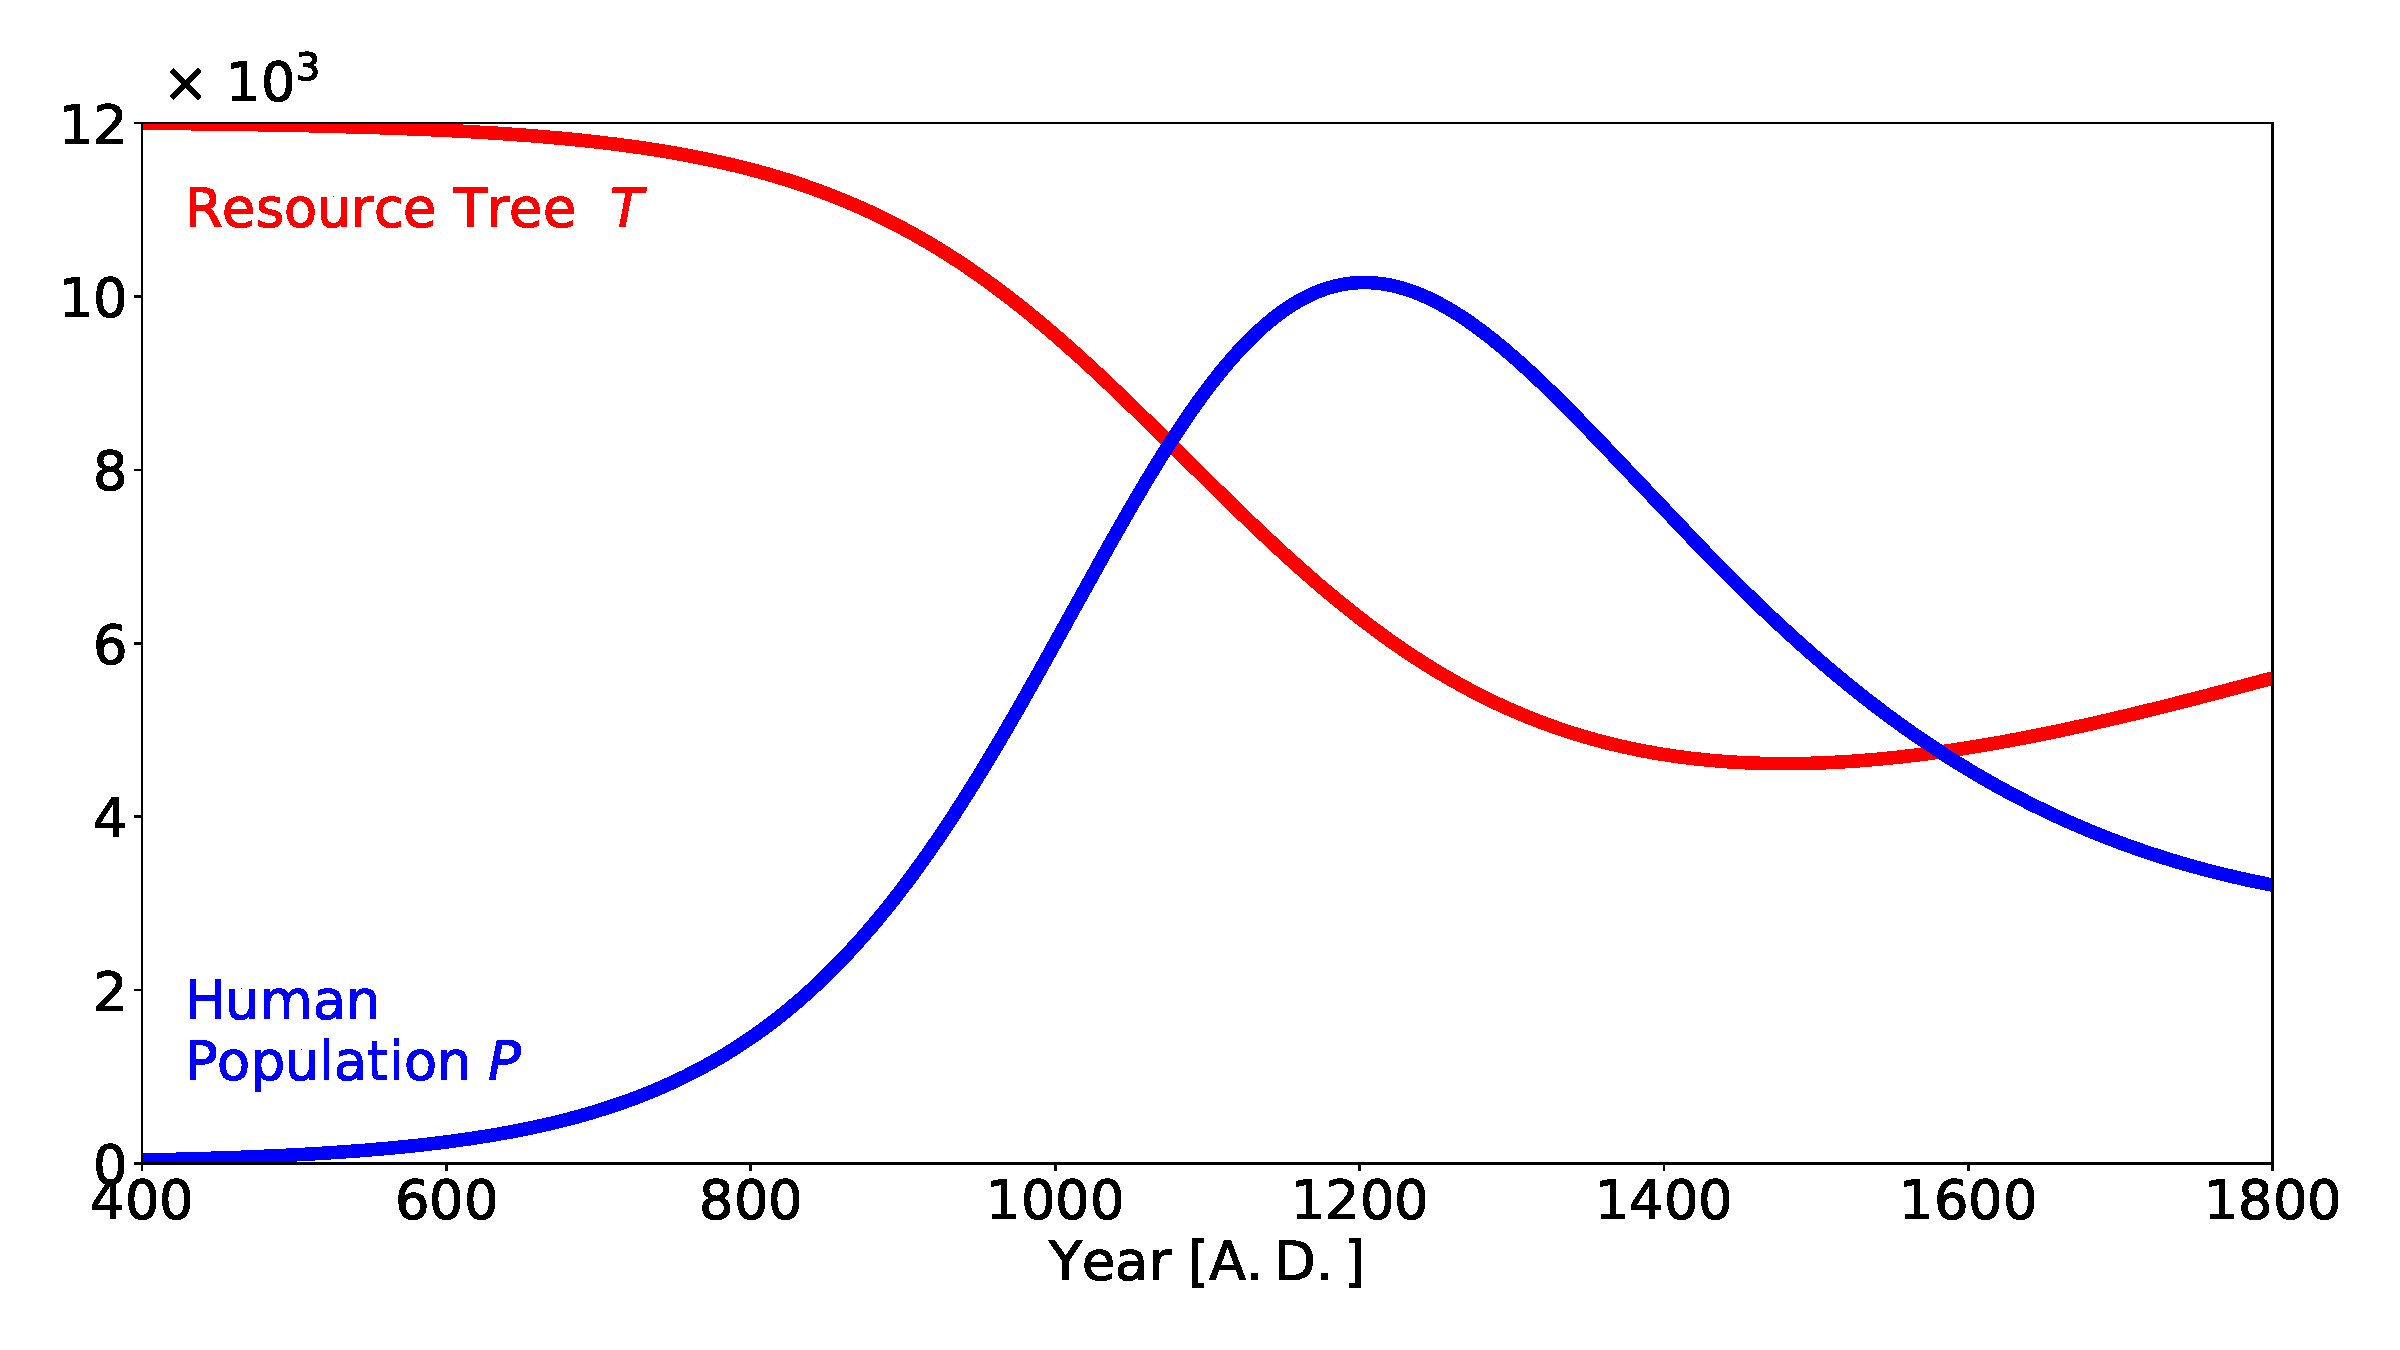
\includegraphics[width=1 \textwidth]{images/Brander1998Model_EI_reduced}
	\caption{Replication of the model in \citet{Brander1998} with parameter setting as in the `Easter Island Base Case' in Figure 3 of the publication. %The dots on the right represent the equilibrium values.
	}
	\label{fig:brander1998eibasecase}
\end{figure}

\paragraph{Extensions of the Basic Model.}
In the last two decades several extensions and adjustments have been added to the first mathematical model by \citet{Brander1998}.
\citet{Reuveny2012} provided an extensive overview of these models.
\citet{Merico2017} additionally summarised gaps and advances within this field of research. 
Here, I point out those models relevant to the word of this thesis.
\citet{dAlessandro2007} separated the single resource into two, one that is inexhaustible and another that is renewable (and irreversibly exhausts if below a certain threshold).
The author found multiple stable states due to this disaggregation of the ecological variable. 
A model by \citet{Good2006} introduced foresight and resource management institutions (either a system of property rights or a social planner).
%to the simple predator-prey harvest in \citet{Brander1998}.
Here, the society's harvest rate is determined by maximising a utility function over a certain time horizon with reasonable discounting (e.g.\ by a social planner, which could be an emergent political hierarchy).
However, the authors found that even with optimal institutions in place, a collapse of the Rapa Nui population is inevitable.
\citet{Basener2008} added another variable to the model next to tree number and human population size, which accounts for the rat population and their devastating impact on tree regrowth as previously found by \citet{Hunt2007}. 
This model was then further extended by a spatial component \citep{Basener2011}. 
A number of homogeneous, one-dimensional cells was defined and diffusion of rats and humans allowed between adjacent cells. 
The authors found that simply changing the mobility of rats can qualitatively alter the dynamics of the human population size.
While this representation is extremely simplified and the diffusion process is unintuitive for human settlement pattern of a small island, this is the only model on Easter Island including a physical space.
Finally, in a recent analysis, \citet{Brandt2015} extended the model of trees, rats, and humans by \citet{Basener2008} with a disease spreading model.
They found that the model can obtain any of the proposed narratives (ecocide, genocide or the slow-demise) through variation of only a few parameters in a reasonable range.
All these models build on the assumptions considered in the macroscopic ODE model by \citet{Brander1998}.


\paragraph{Shortcomings of Macroscopic ODE Models.}
Despite the extensive body of research presented by the numerous macroscopic system models on Easter Island, the dispute between different narratives could not be solved.
The ODE based models, the main tool for Easter Island modelling, typically either showed the same (inherent) boom and bust cycle or showed shortcomings in that different choices of parametrisation (within the uncertainties of the sparse archaeological data) consistently produced contrasting results \citep{Merico2017}.
%ODE-type modelling can only have limited significance.
Next to the uncertainties in the available data to support the assumptions, many shortcomings of these models are inherent problems of macroscopic system modelling.
This includes in particular the missing spatial, microscopic constraints, heterogeneity in the human population, the stochastic nature of the spatial and temporal environment, co-evolving behaviour and emergent phenomena.
A microscopic, agent-based model addresses many of these issues and, therefore, constitutes a useful alternative to macroscopic ODE model approaches as described in the next Section.
%E.g.\ the model by \citet{Brander1998} assumes open access to the resources which defers intuition since the location of an individual restricts the availability of resources. 
%Other models \citep{Good2006} might include a more complex economic which incorporates restrictions on resource harvest but implemented via a social planner.
%Thus, such dynamics are not co-evolving or emergent but externally established 

%While models like \citet{Good2006} have restrictions on the amount of resources, it require a social planner and it is not so much an emergent restriction of the population dyanmics but rather a institution.

\FloatBarrier
\section{Agent-Based Modelling (ABM) of Human-Resource Interactions -- Overview, Motivation and Previous Approaches}
%\begin{itemize}
%\item What is Agent Based Modelling
%\item The basic structure of an ABM in human resource interactions: Agents in environment, Update all agents asynchronously, update environment. Within each update agents change their local environment and their behaviour/properties are in turn influenced by the local environment. 
%\item It breaks with ODE-type of modeling because it enables: 
%\begin{itemize}
%	\item spatially explicit modelling,
%	\item  emergent global behaviour from local rules, 
%	\item computational irreducibility of agent behaviour in terms of crisis. 
%	\item Non-ergodic relation between agents and their environment.
%	\item Stochasticity is natural in the decision making process, due to an agent's imperfect knowledge of the global sitution
%\end{itemize}
%\item ABM in ancient historical population dynamics: Maya \citep{Heckbert2013} and Anasazi \citep{Axtell2002}
%\item Why ABM could help in Easter Island modelling: \citet{Merico2017}.
%\item Structure of this thesis.
%\end{itemize}

\paragraph{Overview of ABM.}
Agent-Based Modelling (ABM) is now a common tool at the centre between cognitive psychology, game theory, and complexity science \citep{Bousquet2004} with roots in the field of Artificial Intelligence.
In Agent-Based Models (ABMs) a system is grown bottom-up from its constituent units.
Hence, an ABM focuses on the microscopic rather than the macroscopic aspects of a system.
The model simulates a number of discrete agents (e.g.\ humans), often situated in an environment, with specific traits.
Agents (and the environment) are updated asynchronously at certain time steps over the simulated period.
In each update, a single agent interacts with the environment and other agents according to a set of rules or heuristics.
These rules are usually heterogeneous, non-linear (e.g.\ discontinuous or discrete), stochastic, time-dependent and adaptive and might be memory- and path-dependent \citep{Bonabeau2002}.
In the case of a spatial model, rules and behaviour additionally depend on the explicit location of an agent in the environment.
Usually, agents make individual decisions, based on perceptions of their local surroundings and their internal state, and thereafter act independently and autonomously.
With this microscopic setup, overall macroscopic dynamics of the system are obtained.
Aggregate system variables can then be interpreted both as outcomes of and as contexts for the agents' decisions and actions \citep{Kohler2000}.
As described in \citet{Bousquet2004}, the mathematical analysis of an ABM, however, is not straight-forward, unless the model is extremely simplified and general.
In fact, validation of an ABM is classically done by simply running simulations (enabled by the rise of computational power in the recent decades), obtaining aggregated system variables and comparing them with observations or testing them for plausibility.

%The field of Agent Based Modelling originally comes from Artificial Intelligence study. 
% WHERE FROM 
% INFORMATICS, EXAMPLES, ...


%These are updated asynchronously in certain timesteps over the simulation period. 
%In each update, a single agent interacts with the environment and other agents and adapts its own features.
%Usually, agents act independently and based on individual decision making by evaluating their state at the current time.
%Aggregate variables of all agents are then a combination of context as well as outcome \citep{Kohler2000}.



\paragraph{Advantages with respect to ODE Models.}
ABMs are applied to study complex systems, i.e.\ systems consisting of multiple components interacting with each other and, thereby, creating feedback loops and non-linearities, because of which the behaviour of the system can not be easily inferred from the input of the model.
%In many complex systems, 
In such systems, ABMs are typically advantageous over macroscopic system models by accounting for the following system properties \citep{Bookstaber2019}:
\begin{itemize}
	\item Emergent phenomena from local, heterogeneous behaviour of the agents,
	\item Computational irreducibility of agent behaviour (e.g.\ in the decision making in times of crisis),
	\item Non-ergodicity of relations between agents and their environment, i.e.\ conditions and rules of behaviour co-evolve with the agent and environment \citep{Kohler2000},
	\item Stochasticity in actions and decision making processes, due to imperfect knowledge or uncertainty of the agents. 
\end{itemize}
Additionally, ABMs allow for a very natural and flexible implementation\footnote{Compare for example with the unintuitive diffusion process in the ODE model by \citet{Basener2011}.} of an explicit space dependency of rules and a spatially heterogeneous environment.
%In ODE models, space dependency is typically implemented via non-intuitive, complex diffusion processes (compare to the model by \citet{Basener2011}).
%In such systems, ABMs are often the most natural and flexible way of describing a system.
%An ABM is especially relevant if a system exhibits emergent phenomena, i.e.\ individual behaviour according to rules cummulates in complex macroscopic patterns.
In particular, if a system exhibits emergent phenomena, crucial information is lost when the heterogeneity of agents is reduced to one representative agent by averaging, as done in macroscopic ODE models \citep{Bonabeau2002}.
Instead, an ABM generates emergence from bottom-up by accounting for non-linear feedbacks due to heterogeneous agents and stochasticity. % e.g.\ connected to uncertainty in the decision making process.

%Furthermore stochastic, discrete processes as in an ABM lead to complex responses of the model outcome, that can not be simply 
% while an ABM gives rise to non-linear feedbacks of fluctuations e.g.\ in the case of uncertainty.
%In such cases, simple averaging and expressing processes by a representative behaviour, as applied in macroscopic system modelling, does not capture emergent phenomena.
%However, an ABM gives rise to non-linear feedbacks from heterogeneous, fluctuating agents e.g.\ in the face of uncertainty and imperfect knowledge in decision making.


\paragraph{Application in Socio-Ecological Systems.}
ABMs have traditionally been applied to problems connected to flows, markets, organisations, or diffusion \citep{Bonabeau2002}.
Typical applications include e.g.\ traffic jams, ant colonies or swarm behaviour of fish and bird flocks.
However, ABMs are also a common approach for socio-ecological systems \citep{Muller-Hansen2017}.
Such a system comprises complex co-evolution of the heterogeneous humans and environment, which interact with each other in non-linear, adaptive ways on multiple time and spatial scales, making it suitable for the application of ABMs \citep{Bousquet2004}.

%The population dynamics of ancient societies 
%, as agents in such a system usually also act heterogeneously and dependent on local space.
%Here, social structure such as the emergence of political organisations in the agent-agent interactions are at the heart of Agent-Based models.
%As agents in ecological systems usually act heterogeneously and strongly dependent on their local environment or neighbourhood, the usage of ABM with an explicit space dependency is suitable \citet{Bousquet2004}.
% motivates the use of ABM in ecological modeling with the local response 

%According to \citet{Bousquet} ABMs in the ecosystem context can be applied to either create scenarios showing `what might be rather than what is' to understand a system or to produce reality-like scenarios in order to test `what if' questions.

%The disadvantage of ABM is that there's no mathematical proof.Bousquet2004.

\paragraph{Application for Ancient Civilisations.}
Agent-Based Modelling has also been applied to study the history of two ancient civilisations.
\citet{Axtell2002} and \citet{Janssen2009}, used an ABM to reproduce the spatio-temporal history of the Anasazi society in a valley in Arizona, US, and its disappearance around $1300\, {\rm A.D.}$. 
Agents in the model represent households with various heterogeneous attributes that interact with the environment via farming. 
The environment is determined from an extensive data record of harvest yield potential in the valley over time and the Agent-Environment interaction is based on this yield and a set of anthropologically plausible rules.
Agents choose a location for a farm depending on the maximum potential yield in a certain distance to water and for the nearest possible settlement with access to water. 
The harvest success determines the fertility and, thus, the dynamics of agent numbers and overall population in the valley.
\citet{Heckbert2013} developed an ABM for the Maya civilisation resulting in a `somewhat analogous' reproduction of the spatial pattern and timeline.
The agents in this model generate a certain amount of agricultural yield on a discretised map based on a benefit-cost assessment. 
They are further connected in clustered, adaptive trade networks, from which they benefit.
Both of these approaches by \citet{Axtell2002} and \citet{Heckbert2013} attempted to explain the spatio-temporal history of an ancient civilisation by developing an Agent-Based Model with anthropological rules and a biologically, geographically explicit environment on a discretised map.


\paragraph{Motivation for Applying an ABM on Easter Island.}
This thesis presents a similar Agent-Based modelling approach for the history of Easter Island.
I have discussed many aspects and advantages of ABM, which apply in socio-ecological systems, and for modelling ancient societies (and Easter Island in particular).
Similar to the valley of the Anasazi, Easter Island is a small, confined space with distinct geographical and biological features with heterogeneous agricultural suitability.
\citet{Merico2017} further argues for the use of an ABM for Easter Island to overcome the shortcomings of ODE models and limits of the available archaeological and palynological data.
The main features of the ABM presented here, thus, include a spatially explicit environment, locally confined agent-environment interaction, a simple adaptation strategy of agents to environmental degradation and individual, stochastic moving decisions by agents.

